\documentclass[12p]{article}
\usepackage[a4paper,left=0.4in, top=1in, bottom=1in]{geometry}
%% The amssymb package provides various useful mathematical symbols
\usepackage{amssymb}
%% The amsthm package provides extended theorem environments
%% \usepackage{amsthm}
%% The bm package lets you access bold symbols in math mode using the \boldsymbol command (useful to get bold greek letters).
\usepackage{bm}
%% The bbm package is contains the indicator function symbol \mathbbm{1}
\usepackage{bbm}
%% The amsmath package contains the split environment, letting you split equations into multiple lines.
%% See "https://www.sharelatex.com/learn/Aligning_equations_with_amsmath " for an explanation.
\usepackage{amsmath}
\usepackage{algorithm}
\usepackage{algpseudocode}
\usepackage{pgf}
\usepackage{tikz}
\usetikzlibrary{mindmap, shadows}
\usepackage{float}
\newfloat{algorithm}{t}{lop}
%% For creating draft watermark
%\usepackage{draftwatermark}
%\SetWatermarkText{DRAFT}
%\SetWatermarkScale{1}
\usepackage{pdfpages}
%\usepackage{textcomp}
%% Declaring \argmin and \argmax operators:
\DeclareMathOperator*{\argmin}{arg\,min}
\DeclareMathOperator*{\argmax}{arg\,max}
%% Declare trace operator \Tr:
\DeclareMathOperator*{\Tr}{Tr}
%% shorthand for \boldsymbol and \overline
\let\bs\boldsymbol
\let\ol\overline
%% command that allows equations to be split across pages
%\allowdisplaybreaks[3]

\begin{document}
\pagenumbering{gobble}
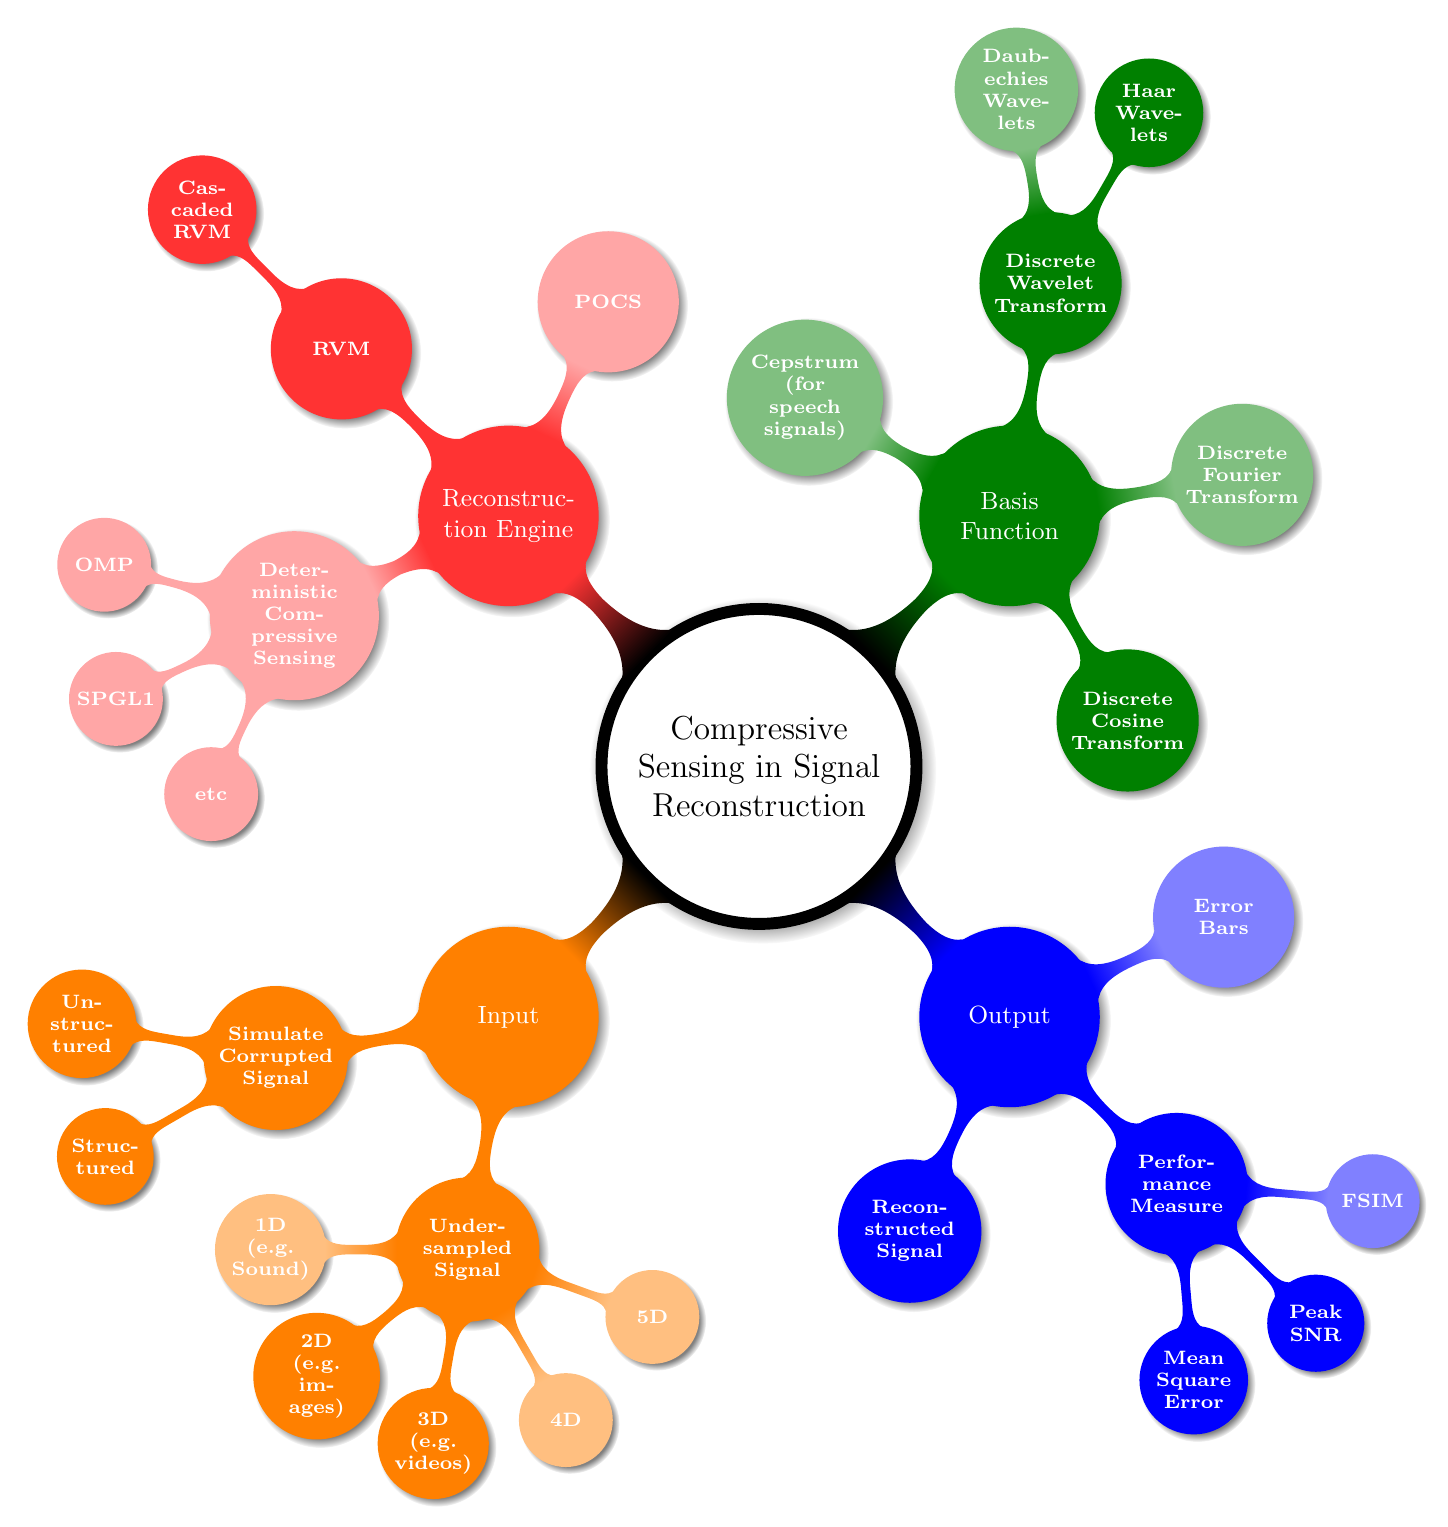
\begin{tikzpicture}[mindmap]
  \begin{scope} [
    every node/.style={concept, circular drop shadow, execute at begin node=\hskip0pt},
    root concept/.append style={
      concept color=black, fill=white, line width=1ex, text=black, font=\large},
    text=white,
    input/.style={concept color=orange, faded/.style={concept color=orange!50}},
    basis/.style={concept color=green!50!black, faded/.style={concept color=green!50!black!50}},
    engine/.style={concept color=red!80!white, faded/.style={concept color=red!50!white!70}},
    output/.style={concept color=blue, faded/.style={concept color=blue!50}},
    grow cyclic,
    level 1/.append style={level distance=4.5cm, sibling angle = 90},
    level 2/.append style={level distance=3cm, font=\bf\scriptsize, sibling angle = 70},
    level 3/.append style={level distance=2.5cm, font=\bf\scriptsize, sibling angle = 40}]
    \node [root concept]{Compressive Sensing in Signal Reconstruction}
      child [input] { node {Input}
        child { node {Simulate Corrupted Signal} 
          child { node {Unstructured} }
          child { node {Structured} }
        }
        child { node {Undersampled Signal} 
          child [faded] { node{1D (e.g. Sound)} }
          child { node{2D (e.g. images)} }
          child { node{3D (e.g. videos)} }
          child [faded] { node{4D} }
          child [faded] { node{5D} }
        }
      }
      child [output] { node {Output} 
        child { node{Reconstructed Signal} }
        child { node{Performance Measure} 
          child { node{Mean Square Error} }
          child { node{Peak SNR} }
          child [faded] { node{FSIM} }
        }
        child [faded] { node{Error Bars} }
      }
      child [basis] { node {Basis Function}
        child { node{Discrete Cosine Transform} }
        child [faded] { node {Discrete Fourier Transform} }
        child { node{Discrete Wavelet Transform} 
          child { node{Haar Wave\-lets} }
          child [faded] { node{Daub\-echies Wave\-lets} }
        }
        child [faded] { node {Cepstrum (for speech signals)} }
      }
      child [engine] { node {Reconstruction Engine} 
        child [faded] { node {POCS} }
        child { node {RVM} 
          child { node {Cascaded RVM} }
        }
        child [faded] { node{Deterministic Compressive Sensing}
          child { node{OMP} }
          child { node{SPGL1} }
          child { node{etc} }
        }
      };
  \end{scope}
\end{tikzpicture}
\vspace{0.2in}

\hspace{0.3in}
\noindent
\fbox{\parbox{3in}{\underline{Speed depends on}
\begin{itemize}
\item Signal Size (-)
\item Block Size (-)
\item Reconstruction Algorithm
\item Cascade Depth (-)
\item Parallelization (blocks are independent)
\end{itemize}}}
\hspace{0.1in}
\fbox{\parbox{3in}{\underline{Accuracy depends on}
\begin{itemize}
\item Basis Function
\item Block Size (+)
\item Reconstruction Algorithm
\item Cascade Depth (+)
\item Level of Corruption
\end{itemize}}}

\end{document}


%% End of file `rvm.tex'.